\chapter{Introduction}

\label{chapter:intro}

Micro unmanned Aerial Vehicles (MAVs, also called drones or Unmanned Aerial Vehicles, UAVs) recently saw a rise in usage across various fields. 
Drones are already widely used in cinematography \cite{Mademlis2020}, advertising \cite{Ullah2021} and agriculture \cite{Kim2019}. 
City emergency departments also use MAVs - firefighters can see and evaluate the situation from the sky, localize the source of fire and put it out \cite{Pritzl2021}.
Another field where MAVs can be used in the nearest future is transportation. 
Fast parcel delivery \cite{She2021} and content transportastions \cite{Gupta2021,Aloqaily2022} are quite promissing fields of MAV application together with smart city concepts evolving \cite{Ortiz2019}.
Nowadays, even collaborative transportation systems are becoming realistic - multi-robot swarming algorithms are better developed, and that allows their usage for the transportation of large objects \cite{Bacelar2020} that one drone alone can not lift. 
MAVs are also widely used in the military industry.

As drones are used so widely, there is a significant demand for an increase in drone-related safety. 
Many commercially available drones are expensive and quite heavy, so that accidents can be costly and dangerous to property and human health. 
Even if a drone is controlled remotely, obstacles can be hard to spot and avoid when the pilot flies far away.
Similar limitations apply to flying in forests or cities (in situations when it is legal, for example - emergency departments and moviemakers can do it), where it may be hard to maintain the line of sight for the pilot.
First-person view glasses may be used in such situations to mitigate these limitations to some degree, but still, only provide limited information about the surrounding environment.
Most of these systems only provide a field of view (FOV) smaller or comparable to the FOV of a human eye (which is approx. a third of the full sphere FOV \cite{humeye}).
In this sense, autonomous robots can sense and avoid obstacles much better, but only if they have a well-designed system running onboard and enough sensors to cover the area around the robot.

Automatic obstacle avoidance systems become especially important in closed environments with many obstacles, such as forests, cities, or indoor environments.
To ensure complete coverage of the surroundings of the MAV for the collision avoidance system, it can be equipped with multiple sensors pointing in all directions.

Considering this context, a compact obstacle avoidance system is a perspective field for research. 
Even though the idea is not new, there is no complete, publicly available visual obstacle avoidance system for MAVs that can cover the whole space around them with few sensors.
One of the best is perhaps the Skydio system\footnote{\href{https://www.skydio.com/skydio-autonomy}{Skydio autonomy: https://www.skydio.com/skydio-autonomy }} which has six 4k \ang{200} navigation cameras, and neural networks are used for the mapping, obstacle avoidance and path planning \cite{Skydio}. 
It is available only for the US military.
The DJI Mavic 3 drone\footnote{\href{https://www.dji.com/cz/mavic-3}{DJI Mavic 3: https://www.dji.com/cz/mavic-3}} seems to be a better solution with eight cameras and an infrared sensor at the bottom.
Unfortunately, neither of these companies provide any scientific publications, system specifications or implementation details, so we can only conclude from the limited available information.

\begin{figure}[t]
    \centering
    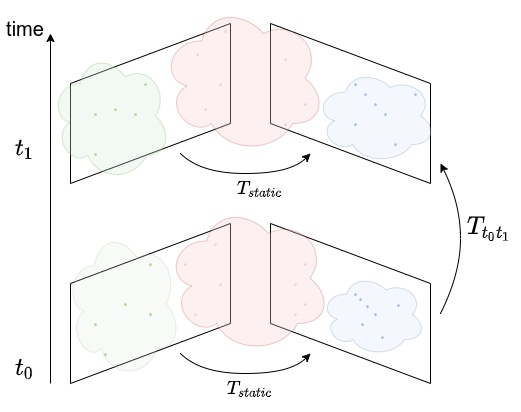
\includegraphics[width=0.6\textwidth]{graphics/general_scheme.png}
    \caption{ A general scheme of the multi-camera obstacle detection problem.}
    \label{fig:intro_general}
\end{figure}

\autoref{fig:intro_general} presents a scheme of the proposed system.
In the figure, $T_{static}$ is the transformation between two cameras mounted onboard the MAV.
$T_{static}$ is obtained with stereo pair calibration. 
At time $t_0$, a new pair of images is captured by the cameras.
A feature detector extracts points of interest from the images.
Points that lie in the part of the images corresponding to a section of the cameras' field of view that overlaps are then selected (the red point cloud in \autoref{fig:intro_general}), and correspondence matches between these points from the two images are found based on their feature descriptors.
A calibrated projection model of the cameras and the transformation $T_{static}$ are used to estimate 3D points from the matched point pairs.
Then at time $t_1$, when a new pair of images is received, the same process is repeated. 
In parallel, an incremental Structure from Motion (SfM) algorithm processes sequences of images from each camera separately to estimate 3D points corresponding to nearby objects in the environment. However, monocular SfM algorithms can generally only estimate the environment up to an unknown scaling factor \cite{SfM}. To address this problem, the red point cloud is used to find the scale of the points obtained using the SfM algorithm from images captured at $t_0$ and $t_1$ (the blue and green point clouds in \autoref{fig:intro_general}).

\section{Related Works}

There are many approaches to tackling MAV obstacle avoidance in the published literature using various sensors.
In most articles, a stereo pair of two parallel cameras looking in the same direction (classical stereo pair) \cite{Lin2021,Ruf2018,Oleinikova2015,Back2020} are used for that, but there are also approaches relying on monocular vision \cite{Mejias2010,Zhang2019,Bills2011} or 2D or 3D Light Detection and Ranging (LiDAR) sensors \cite{Ramasamy2016}.
Distance sensors relying on ultrasonic sound waves and time of flight sensors have low accuracy and are sensitive to noise, which is why they are typically not used alone but in combinations with other sensors \cite{Gageik2015, Nor2017}. 
There are also convolutional neural network-based approaches for depth estimation from monocular cameras \cite{Zhang2019,Yu2013, Park2020} and from stereo cameras \cite{Back2020}.

These sensors have various advantages and shortcomings, making them suitable for different applications \cite{Huang2019, Aguilar2017}.
3D LiDARs are relatively heavy and expensive but can provide good precision and a 3D coverage of the environment.
2D LiDARs, which are typically more lightweight and significantly cheaper, have successfully been deployed on ground vehicles. 
However, they are not as suitable for onboard deployment on MAVs because, unlike ground vehicles, MAVs can have three degrees of translational movement, so a 2D LiDAR cannot cover all possible directions of movement, making it unsuitable for robust collision avoidance.
Stereo camera sensors are generally more expensive and complex than monocular cameras but can provide precise depth images. 
Industrial stereo cameras typically come with a software development toolkit (SDK) and programming libraries, they are already calibrated from the factory and ready to be deployed and used, which makes them more user-friendly than a custom made stereo pair. 
However, it is infeasible to alter the hardware specifications in most cameras, for example, changing FOV or camera lenses.
Such hardware limitations make it challenging to use in some research applications.
As already mentioned, ultrasonic and infrared sensors have a low precision, relatively short range, and are sensitive to noise.
However, they are often used because they are relatively small, cheap and light.

\begin{figure}[h]
    \begin{subfigure}[h]{0.31\textwidth}
      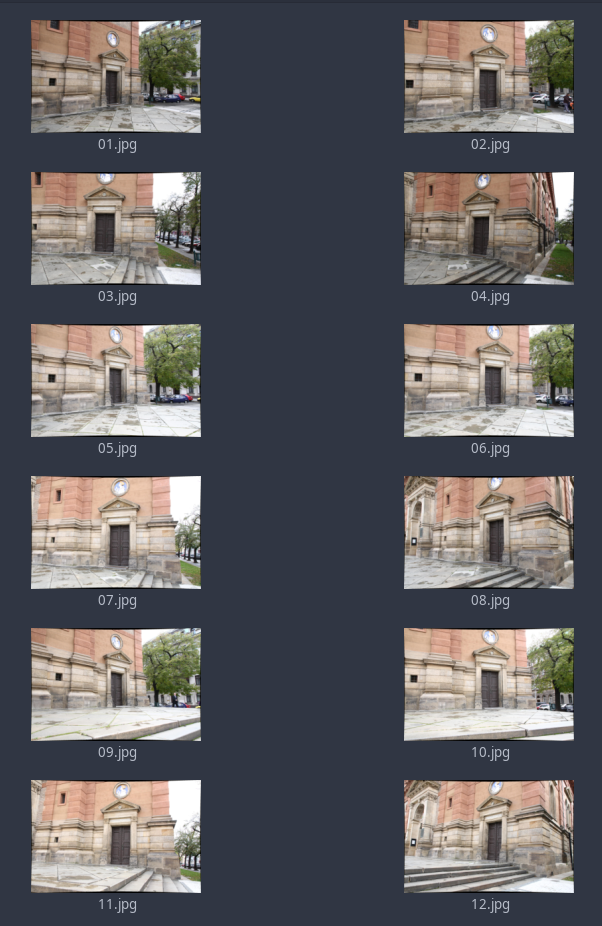
\includegraphics[width=\textwidth]{graphics/input_set.png}
      \caption{Input images.}
      \label{fig:pc_input}
    \end{subfigure}
    \hfill
    \begin{subfigure}[h]{0.65\textwidth}
      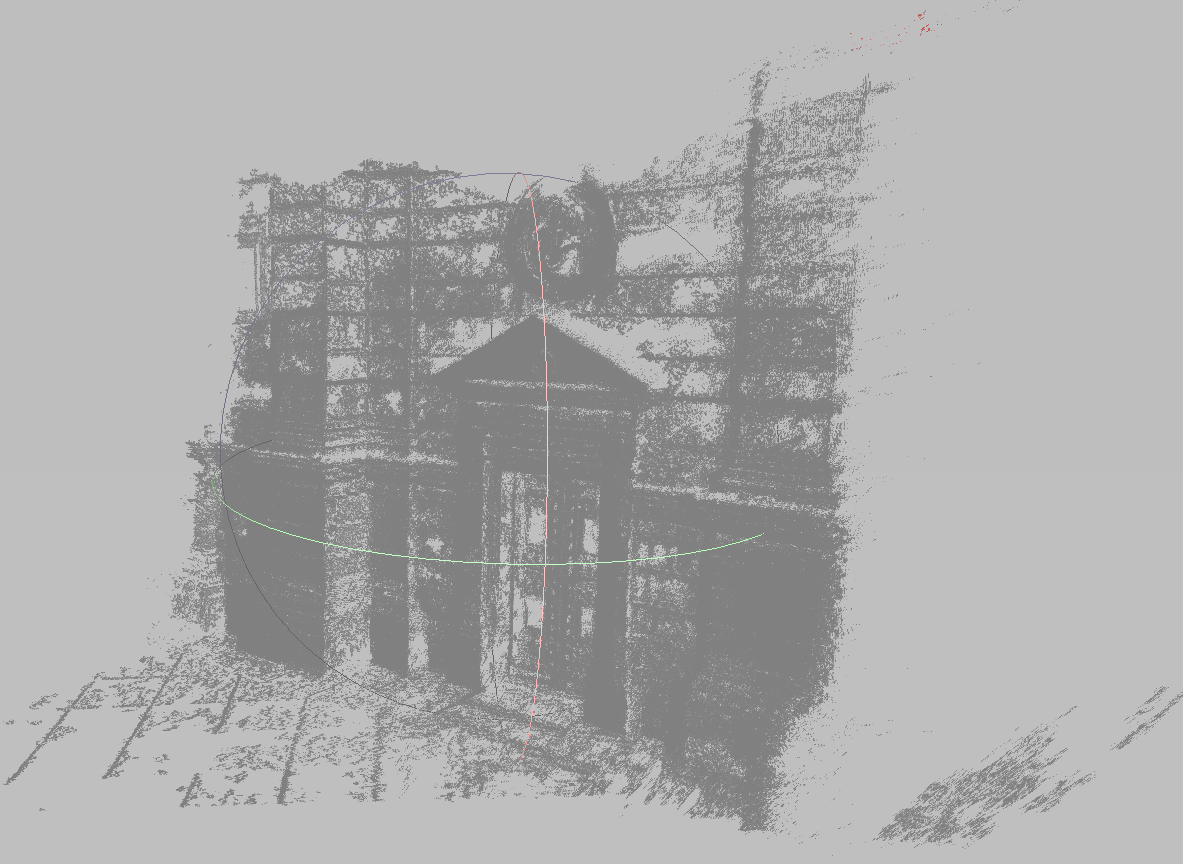
\includegraphics[width=\textwidth]{graphics/reconstructed.png}
      \caption{Output of an SfM algorithm.}
      \label{fig:pc_output}
    \end{subfigure}
    \caption[Ilustration of Structure from Motion.]{Ilustration of Structure from Motion, source - \url{https://github.com/Myralllka/CTU_3d_computer_vision/}}
    \label{fig:pc_recons}
\end{figure}

Real-time Simultaneous Localization And Mapping (SLAM) systems can also be used for obstacle avoidance \cite{Moreno2014}. 
These problems are closely related. 
SLAM keeps track of the robot's position while constructing and updating a map of an unknown environment. 
At the same time, obstacle avoidance is a problem of detecting and avoiding the nearest obstacles in an unknown environment to keep the robot safe from harmful collisions.
Both problems are related to making a 3D map of an unknown environment, but the precision of distance measurements to the nearest objects is much more critical for obstacle avoidance.
Sometimes SLAM can be a considerable overhead because it usually includes saving, updating the map, and robot localization in the map, while obstacle avoidance only needs real-time information about the robot's surrounding.

Structure from Motion (SfM) is another family of algorithms that may be used to implement a system for avoiding obstacles. 
SfM is a method of 3D reconstruction from a continuous sequence of images as illustrated in \autoref{fig:pc_recons}.
Using this approach, a dense point cloud as in \autoref{fig:pc_output} can be computed, and obstacles can be detected \cite{Lee2008}. 
This algorithm alone has multiple problems.
Firstly, it can not recover information about such parts of an image as the robot's shadow or any other object moving with the same velocity in the same direction as the camera.
Secondly, it requires images from at least two different views to work.
If there are moving objects, their correct position relative to a moving camera can not be obtained.
These problems can be tackled by combining SfM with other algorithms.

\section{Problem definition}
\label{sec:problem_definition}
This thesis aims to design a visual obstacle avoidance system for MAVs, create a physical device implementing the system and measure its performance. 
The proposed solution assumes an MAV with a limited size and lifting force that constrains the number, weight and size of its onboard sensory equipment. 
The MAV is thus equipped with two calibrated cameras with a known transformation between them. 
The fields of view of the cameras overlap enough to detect close obstacles.
Framerate of the cameras is sufficient to operate in real-time, and the frames are synchronized in time.
The MAV is also equipped with an onboard computer with enough computational power to process the images at a rate sufficient for obstacle avoidance.
The flight environment is assumed to be well-lit and contains objects with well-distinguishable visual features that the cameras can observe.
These features should be unique so that the same feature can be unambiguously matched in images from the two cameras.
The expected output is a reconstruction of the 3D environment around the drone in the form of a set of points representing the nearest objects.
Depending on the estimated distance, these are the possible obstacles that should be avoided.
The system can be integrated with the MAV control system to provide obstacles, so the solution working rate on the MAV's hardware should be sufficient for agile manoeuvering and obstacle avoidance.

